\hspace{3mm}

\begin{wrapfigure}{r}{0.25\linewidth}
    \centering
    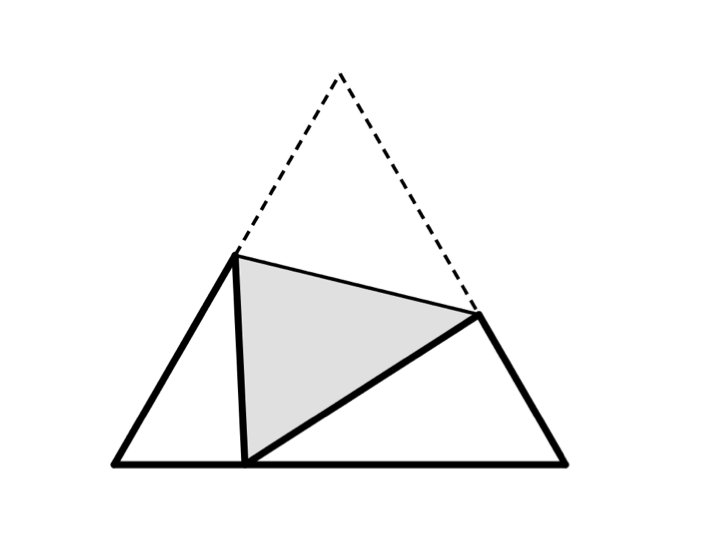
\includegraphics[width=\linewidth]{VII блок/Киви/lesson_1/Task_1.png}
\end{wrapfigure}

\centerline{\Huge \bf  Движения плоскости}
\centerline{\Huge \bf Центральная и осевая симметрии}

\begin{flushright}
    \scriptsize{}
\end{flushright}

\hspace{3mm}

\problem{1} Бумажный равносторонний треугольник перегнули по прямой так, что одна из вершин попала на противоположную сторону (см. рисунок). Докажите, что углы двух белых треугольников соответственно равны.

\problem{2} На продолжении диагонали $AC$ квадрата $ABCD$ за точку $C$ выбрана точка $X$ так, что $BX$ = $AC$. Найдите угол $\angle AXB$

\problem{3} На диагонали $AC$ квадрата $ABCD$ выбраны точки $XY$ и $Y$ так, что точка $Y$ лежит на отрезке $CX$ и $XY = YD$. Известно, что $\angle XBC = \alpha $. Чему равен $\angle XYD$?

\begin{wrapfigure}{r}{0.2\linewidth}
    \centering
    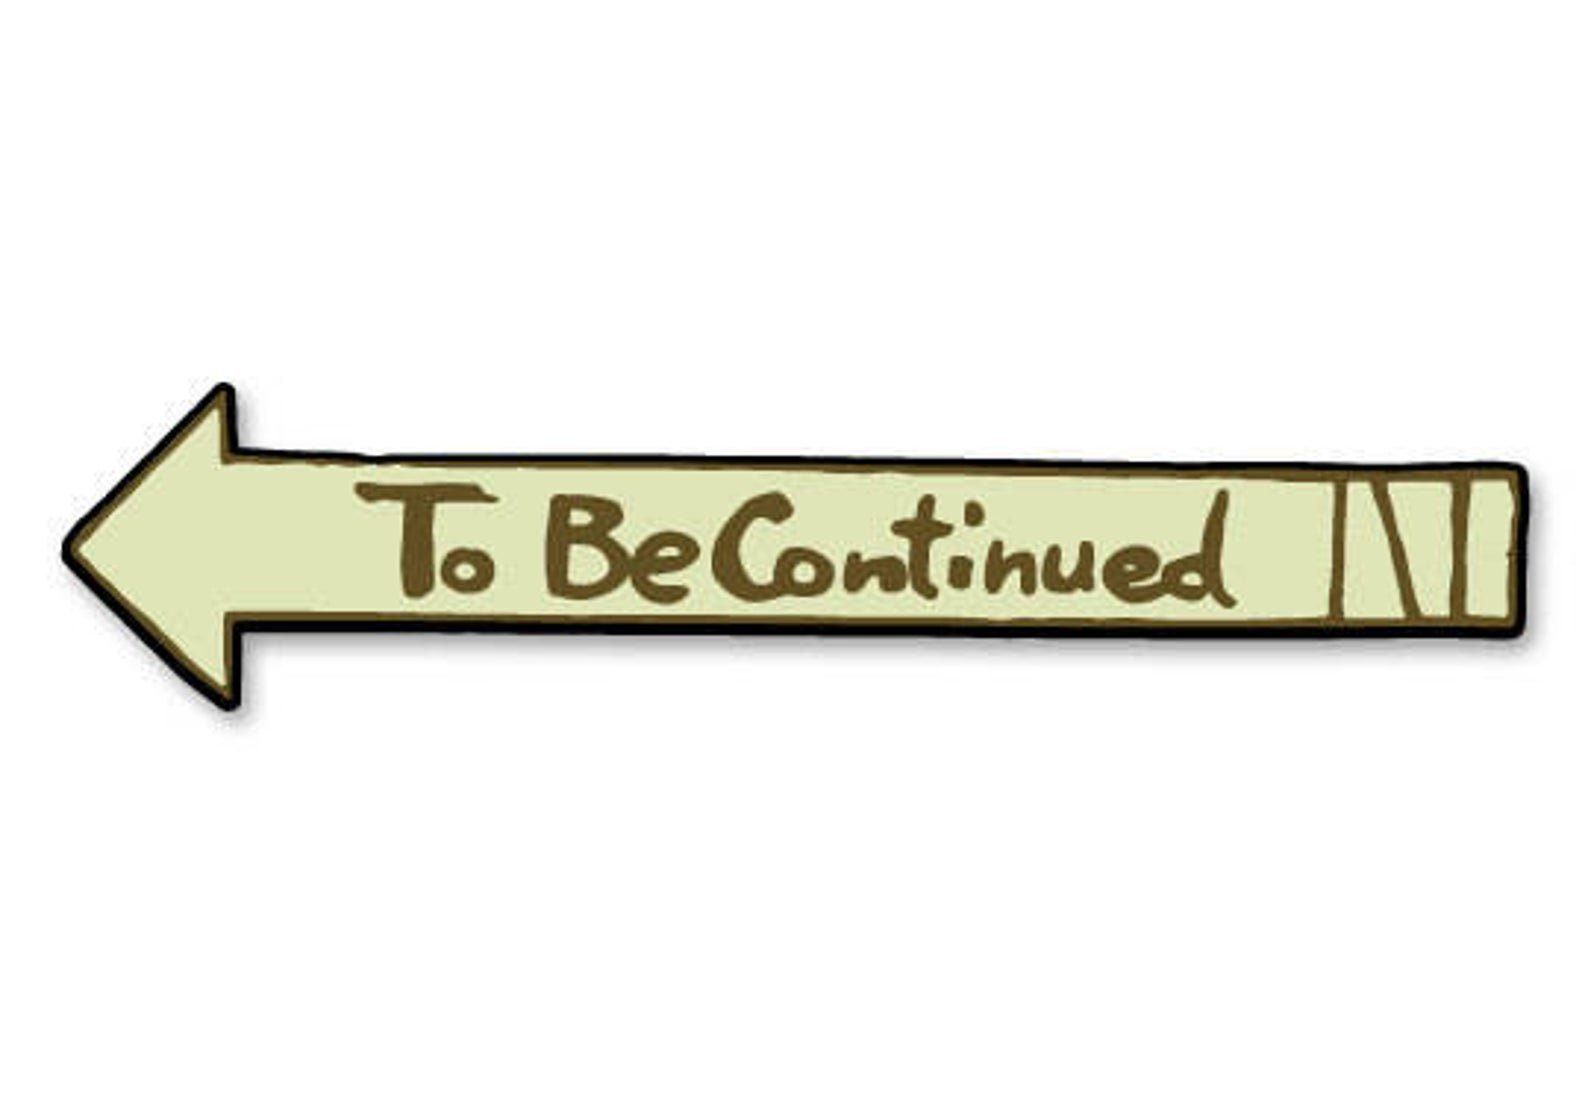
\includegraphics[width=\linewidth]{VII блок/Киви/lesson_1/to_be_continued.jpeg}
\end{wrapfigure}

\problem{4} На стороне $BC$ треугольника $ABC$ выбрали точки $P$ и $Q$ такие, что $BA$ = $BP$ и $CA = CQ$ . Точка $I \ -$  точка пересечения биссектрис треугольника $ABC$. Докажите, что треугольник $IPQ$ равнобедренный.